\paragraph{Sơ đồ tuần tự luồng đàm thoại trực tiếp với AI bằng giọng nói}

Luồng nghiệp vụ này mô tả
phiên giọng nói voice.
Voice Agent trong Chatbot Service nhận audio,
đọc metadata từ participant,
resolve persona để cập nhật DynamicTTS,
gọi công cụ RAG,
sau đó phát audio phản hồi qua LiveKit.

\begin{figure}[H]
\centering
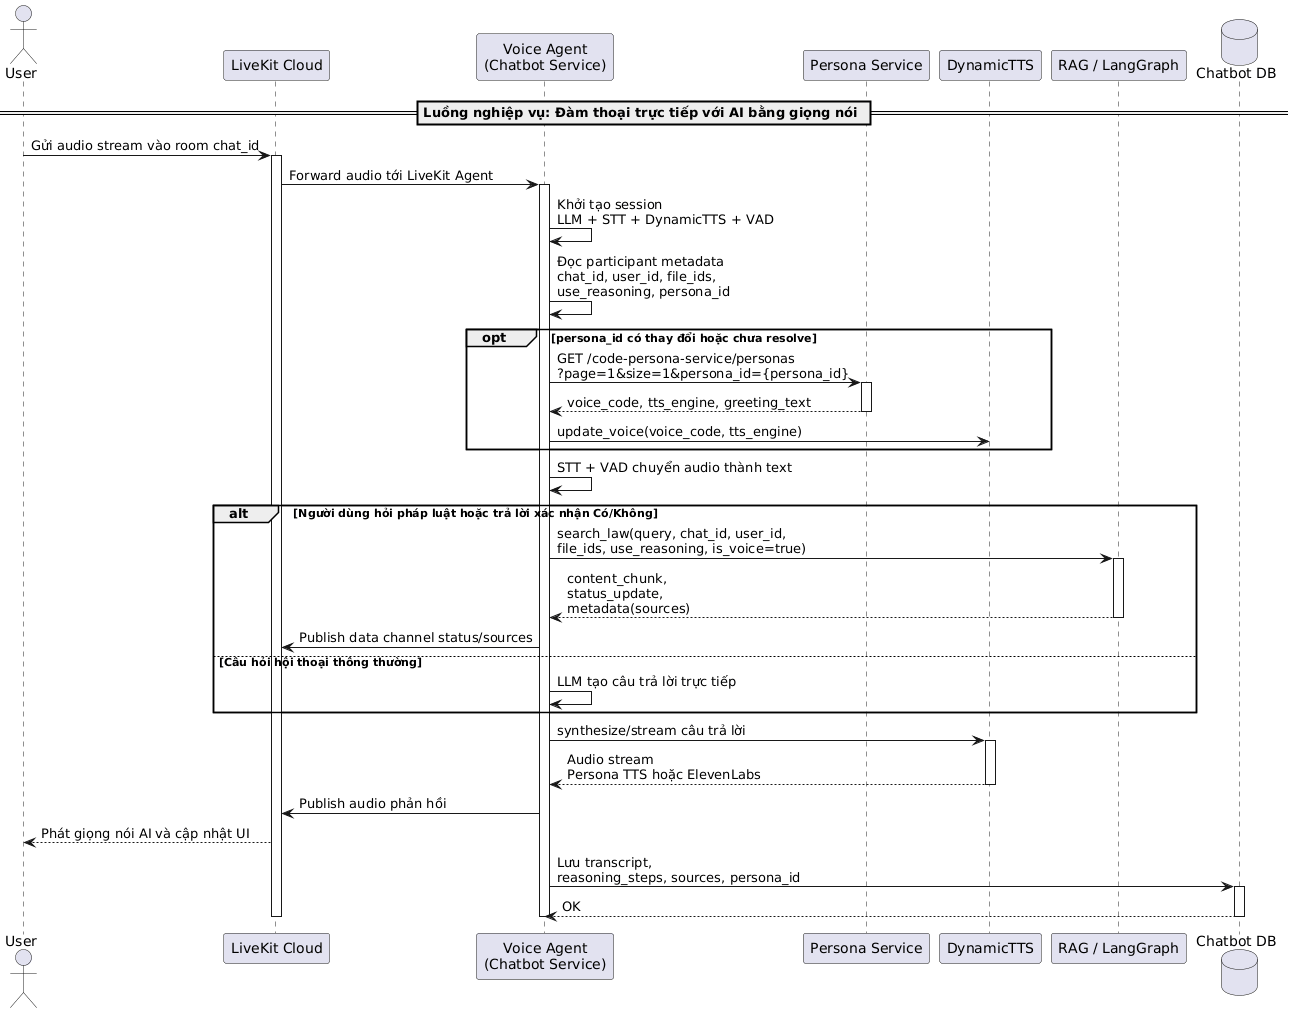
\includegraphics[width=0.95\textwidth]{contents/Sequence/UML-Sequence-UserVoiceChatWithAi.png}
\caption{Sơ đồ tuần tự luồng đàm thoại trực tiếp với AI bằng giọng nói}
\end{figure}

\subparagraph{Mô tả tổng quan}

\begin{itemize}

\item \textbf{Nhận thông tin đàm thoại:}
Bộ xử lý đàm thoại giọng nói
nhận thông tin phòng họp thời gian thực của người dùng
bao gồm định danh cuộc trò chuyện, định danh người dùng, danh sách tài liệu phân tích, tùy chọn lập luận nâng cao và định danh nhân vật.

\item \textbf{Cấu hình nhân vật:}
Khi nhân vật được thay đổi, bộ xử lý gọi địa chỉ nhân vật công khai
để lấy định danh giọng nói
và cấu hình công cụ
chuyển đổi văn bản thành giọng nói,
sau đó cập nhật giọng nói cho bộ phát âm thanh.

\item \textbf{Nhận dạng giọng nói:}
Bộ phận nhận dạng giọng nói
chuyển âm thanh nói
của người dùng thành văn bản.
Nếu câu hỏi liên quan
đến pháp luật
hoặc là phản hồi xác nhận thông tin,
bộ xử lý sẽ kích hoạt công cụ RAG.

\item \textbf{Tìm kiếm tài liệu và luật:}
Công cụ RAG tìm kiếm tài liệu kết hợp thông tin tài liệu cá nhân
và nguồn luật để xếp hạng, kiểm tra hiệu lực văn bản, tổng hợp lập luận
và trả về kết quả từng phần bao gồm cập nhật trạng thái
và nguồn tài liệu tham khảo qua kênh truyền dữ liệu của phòng họp.

\item \textbf{Phát âm thanh phản hồi:}
Câu trả lời dạng văn bản được chuyển thành tệp âm thanh
bằng công cụ chuyển đổi giọng nói
và phát lại phòng họp thời gian thực cho người dùng nghe,
đồng thời nội dung văn bản cuộc trò chuyện
được lưu trữ vào CSDL chatbot.
\end{itemize}

\begin{table}[H]
\centering
\renewcommand{\arraystretch}{1.3}

\begin{tabular}{|l|l|p{5cm}|}
\hline
\textbf{Thành phần} & \textbf{Phân loại} & \textbf{Vai trò trong hệ thống} \\ \hline
User & Actor & Người dùng nói chuyện trực tiếp với AI. \\ \hline
LiveKit Cloud & External Service & Chuyển tiếp audio và data channel giữa client và Voice Agent. \\ \hline
Voice Agent & Component & Xử lý STT/VAD, gọi tool RAG, xuất bản trạng thái và lưu transcript. \\ \hline
Persona Service & Microservice & Cung cấp TTS và thông tin persona. \\ \hline
DynamicTTS & Component & Chọn TTS theo engine hiện tại: Persona TTS qua API OpenAI-compatible hoặc ElevenLabs. \\ \hline
RAG / LangGraph & AI Pipeline & Tra cứu pháp luật, tài liệu cá nhân và sinh trạng thái reasoning. \\ \hline
Chatbot DB & Database & Lưu transcript, reasoning steps, sources và persona. \\ \hline
\end{tabular}
\caption{Các thành phần tham gia luồng đàm thoại trực tiếp với AI bằng giọng nói}
\end{table}
